\chapter{Basic Geometric Algebra}
\section{Axioms of Geometric Algebra}
Let $\Vsp\lp p,q\rp$ be a finite dimensional vector space of signature 
$\lp p,q\rp$\footnote{To be completely general we would have to consider $\Vsp\lp p,q,r\rp$ 
where the dimension of the vector space is $n=p+q+r$ and $p$, $q$, and $r$ are the number of basis
vectors respectively with positive, negative and zero squares.} over $\Re$. Then
$\forall a,b,c \in \Vsp$ there exists a geometric product with the
properties - \\
\benn
\begin{array}{c}
(ab)c = a(bc) \\
a(b+c) = ab+ac \\
(a+b)c = ac+bc \\
aa \in \Re
\end{array}
\eenn
If $a^{2} \ne 0$ then $a^{-1} = \bfrac{1}{a^{2}}a$.
\section{Why Learn This Stuff?}
The geometric product of two (or more) vectors produces something ``new'' like
the $\sqrt{-1}$ with respect to real numbers or vectors with respect to scalars.  
It must be studied in terms of its effect on vectors and in terms of its 
symmetries. It is worth the effort.  Anything that makes understanding rotations
in a $N$ dimensional space simple is worth the effort! Also, if one proceeds on
to geometric calculus many diverse areas in mathematics are unified and many areas
of physics and engineering are greatly simplified.
\section{Inner, $\cdot$, and outer, $\w$, product of two vectors and their basic
properties}
The inner (dot) and outer (wedge) products of two vectors are defined by
\be
a\cdot b \equiv \half\lp ab+ba \rp
\ee
\be
a\w b \equiv \half\lp ab-ba \rp
\ee
\be
ab = a\cdot b+a\w b
\ee
\be
a\w b = -b\w a
\ee
\be
\begin{array}{c}
c = a+b \\
c^{2} = \paren{a+b}^{2} \\
c^{2} = a^{2}+ab+ba+b^{2} \\
2a\cdot b = c^{2}-a^{2}-b^{2} \\
a \cdot b \in \Re
\end{array}
\ee
\be
a \cdot b = \abs{a}\abs{b}\cosf{\theta} \mbox{ if } a^{2},b^{2}> 0
\ee
Orthogonal vectors are defined by $a\cdot b = 0$. For orthogonal vectors $a\w b = ab$. Now compute $\lp a\w b \rp^{2}$
\begin{align}
\lp a\w b \rp^{2} &= -\lp a\w b \rp\lp b\w a \rp \\
                  &= -\lp ab - a\cdot b \rp\lp ba - a\cdot b \rp \\
                  &= -\lp abba -\lp a\cdot b\rp\lp ab+ba \rp + \lp a\cdot b \rp^{2}\rp \\
                  &= -\lp a^{2}b^{2} - \lp a\cdot b \rp^{2}\rp \\
                  &= - a^{2}b^{2}\lp 1 - \cos^{2}\lp\theta \rp \rp \\
                  &= - a^{2}b^{2}\sin^{2}\lp\theta \rp
\end{align}
Thus in a Euclidean space, $a^{2},b^{2} > 0$, $\lp a \w b \rp^{2} \le 0$ and $a \w b$ is proportional
to $\sinf{\theta}$.
If $\epar$ and $\eperp$ are any two orthonormal unit vectors in a Euclidean space then $\lp\epar\eperp\rp^{2} = -1$. Who
needs the $\sqrt{-1}$?

\section{Outer, $\w$, product for $r$ Vectors in terms of the geometric product}
Define the outer product of $r$ vectors to be ($\varepsilon^{\vprod{i_{1}}{i_{r}}}_{\vprod{1}{r}}$ is the mixed permutation symbol)
\be\label{eq13}
\wprod{a_{1}}{a_{r}} \equiv \bfrac{1}{r!}\Sum{i_{1}}{i_{r}}
     \varepsilon^{\vprod{i_{1}}{i_{r}}}_{\vprod{1}{r}}
     \vprod{a_{i_{1}}}{a_{i_{r}}}
\ee
Thus
\begin{align}
\wprodi{a_{1}}{\paren{a_{j}+b_{j}}}{a_{r}} &=   \nonumber \\
    & \hspace{-1in}\wprodi{a_{1}}{a_{j}}{a_{r}}+
     \wprodi{a_{1}}{b_{j}}{a_{r}}
\end{align}
and
\begin{align}
\wprodi{a_{1}}{a_{j}\w a_{j+1}}{a_{r}} & =  \nonumber \\
  & \hspace{-1in}   -\wprodi{a_{1}}{a_{j+1}\w a_{j}}{a_{r}}
\end{align}
The outer product of $r$ vectors is called a blade of grade $r$.
\section{Alternate Definition of Outer, $\w$, product for $r$
Vectors}

Let $e_{1},e_{2},\dots,e_{r}$ be an orthogonal basis for the set of 
linearly independent vectors $a_{1},a_{2},\dots,a_{r}$ so that we can
write
\be\label{eq16}
	a_{i} = \sum_{j}\alpha_{ij}e_{j}
\ee
Then
\begin{align}
	a_{1}a_{2}\dots a_{r} & =  \paren{\sum_{j_{1}}\alpha_{1j_{1}}
				   e_{j_{1}}} 
	\paren{\sum_{j_{2}}\alpha_{2j_{2}}e_{j_{2}}}
	\dots\paren{\sum_{j_{r}}\alpha_{rj_{r}}
	e_{j_{r}}} \nonumber \\
	& = \Sum{j_{1}}{j_{r}}\alpha_{1j_{1}}\alpha_{2j_{2}}\dots\alpha_{rj_{r}}
	      e_{j_{1}}e_{j_{2}}\dots e_{j_{r}} \label{eq17}
\end{align}

Now define a blade of grade $n$ as the geometric product of $n$ orthogonal vectors. Thus the 
product $e_{j_{1}}e_{j_{2}}\dots e_{j_{r}}$ in equation~\ref{eq17}
could be a blade of grade $r$, $r-2$, $r-4$, etc. depending upon the number of repeated factors.

If there are no repeated factors in the product we have that
\be
	e_{j_{1}}\dots e_{j_{r}} = \varepsilon^{\vprod{j_{1}}{j_{r}}}_{\vprod{1}{r}}
        e_{1}\dots e_{r}		
\ee
Due to the fact that interchanging two adjacent orthogonal vectors in the geometric
product will reverse the sign of the product and we can define the outer product of 
$r$ vectors as
\begin{align}
\wprod{a_{1}}{a_{r}} & = \Sum{j_{1}}{j_{r}}\varepsilon^{\vprod{j_{1}}{j_{r}}}_{\vprod{1}{r}} 
                           \vprod{\alpha_{1j_{1}}}{\alpha_{rj_{r}}}e_{1}\dots e_{r} \label{eq19}\\
		     & = \det\paren{\alpha}e_{1}\dots e_{r}
\end{align}
Thus the outer product of $r$ independent vectors is the part of the geometric product
of the $r$ vectors that is of grade $r$. Equation~\ref{eq19} is equivalent to equation~\ref{eq13}.
This can be proved by substituting equation~\ref{eq17} into equation~\ref{eq13} to get
\begin{align}
	\hspace{-24pt}\wprod{a_{1}}{a_{r}} & =
        \bfrac{1}{r!}\Sum{i_{1}}{i_{r}}\Sum{j_{1}}{j_{r}}\varepsilon^{\vprod{i_{1}}{i_{r}}}_{\vprod{1}{r}} 
	\vprod{\alpha_{i_{1}j_{1}}}{\alpha_{i_{r}j_{r}}}\vprod{e_{j_{1}}}{e_{j_{r}}}\\
	\hspace{-24pt} & =
	\bfrac{1}{r!}\Sum{i_{1}}{i_{r}}\Sum{j_{1}}{j_{r}}\varepsilon^{\vprod{i_{1}}{i_{r}}}_{\vprod{1}{r}}
	\varepsilon^{\vprod{j_{1}}{j_{r}}}_{\vprod{1}{r}}  
	\vprod{\alpha_{i_{1}j_{1}}}{\alpha_{i_{r}j_{r}}}\vprod{e_{1}}{e_{r}} \label{eq22}\\
	\hspace{-24pt} & =
	\bfrac{1}{r!}\Sum{j_{1}}{j_{r}}\varepsilon^{\vprod{j_{1}}{j_{r}}}_{\vprod{1}{r}}
	\varepsilon^{\vprod{j_{1}}{j_{r}}}_{\vprod{1}{r}}  
	\det\paren{\alpha}\vprod{e_{1}}{e_{r}} \label{eq23}\\
	\hspace{-24pt} & = \det\paren{\alpha}\vprod{e_{1}}{e_{r}} \label{eq24}\
\end{align}
We go from equation~\ref{eq22} to equation~\ref{eq23} by noting that 
${\displaystyle\Sum{i_{1}}{i_{r}}\varepsilon^{\vprod{i_{1}}{i_{r}}}_{\vprod{1}{r}}\vprod{\alpha_{i_{1}j_{1}}}
{\alpha_{i_{r}j_{r}}}}$ is just $\det\paren{\alpha}$ with the columns permuted.
Multiplying $\det\paren{\alpha}$ by $\varepsilon^{\vprod{j_{1}}{j_{r}}}_{\vprod{1}{r}}$ 
gives the correct sign for the determinant with the columns permuted.  

If $e_{1},\dots,e_{n}$ is an orthonormal basis for vector space the unit psuedoscalar is defined as
\be
	I = \vprod{e_{1}}{e_{n}}
\ee
In equation~\ref{eq24} let $r=n$ and the $a_{1},\dots,a_{n}$ be another orthonormal basis for the vector space.
Then we may write
\be
	\vprod{a_{1}}{a_{n}} = \det\paren{\alpha}\vprod{e_{1}}{e_{n}}
\ee
Since both the $a$'s and the $e$'s form orthonormal bases the matrix $\alpha$ is orthogonal and 
$\det\paren{\alpha} = \pm 1$.  All psuedoscalars for the vector space are identical to within a
scale factor of $\pm 1$.\footnote{It depends only upon the ordering of the basis vectors.}
Likewise $\wprod{a_{1}}{a_{n}}$ is equal to $I$ times a scale factor.

\section{Useful Relation's}
\begin{enumerate}
\item For a set of r orthogonal vectors, $\mset{e_{1}}{e_{r}}$
\be
\wprod{e_{1}}{e_{r}} = \vprod{e_{1}}{e_{r}}
\ee
\item For a set of r linearly independent vectors, $\mset{a_{1}}{a_{r}}$, there exists
a set of r orthogonal vectors, $\mset{e_{1}}{e_{r}}$, such that
\be\label{17}
\wprod{a_{1}}{a_{r}} = \vprod{e_{1}}{e_{r}}
\ee
If the vectors, $\mset{a_{1}}{a_{r}}$, are not linearly independent then
\be
\wprod{a_{1}}{a_{r}} = 0
\ee
\end{enumerate}
The product $\wprod{a_{1}}{a_{r}}$ is call a ``blade'' of grade $r$. The
dimension of the vector space is the highest grade any blade can have.
\section{Projection Operator}
A multivector, the basic element of the geometric algebra, is made of of a sum of
scalars, vectors, blades. A multivector is homogeneous (pure) if all the blades in 
it are of the same grade.  The grade of a scalar is $0$ and the grade of a vector is
$1$. The general multivector $A$ is decomposed with the grade projection operator
$\proj{A}{r}$ as (N is dimension of the vector space):
\be
A = \sum_{r=0}^{N}\proj{A}{r}
\ee
As an example consider $ab$, the product of two vectors. Then
\be
ab = \proj{ab}{0}+\proj{ab}{2}
\ee
We define $\proj{A}{} \equiv \proj{A}{0}$ for any multivector $A$

\section{Basis Blades}\label{sect_Basis_Blades}
The geometric algebra of a vector space, $\Vsp\paren{p,q}$, is denoted $\GA{p,q}$ 
or $\GA{\Vsp}$ where $\paren{p,q}$
is the signature of the vector space (first $p$ unit vectors square to $+1$ and 
next $q$ unit vectors square to $-1$, dimension of the space is $p+q$). Examples are:

\begin{center}
\begin{tabular}{ccl} \\
$p$ & $q$ & Type of Space \\ \hline 
 3  &  0  & 3D Euclidean \\
 1  &  3  & Relativistic Space Time \\
 4  &  1  & 3D Conformal Geometry
\end{tabular}
\end{center}

If the orthonormal basis set of the vector space is $\mset{e_{1}}{e_{N}}$, the 
basis of the geometric algebra (multivector space) is formed from the geometric
products (since we have chosen an orthonormal basis, $e_{}i^{2}=\pm 1$) of the basis vectors. For
grade $r$ multivectors the basis blades are all the combinations of basis
vectors products taken $r$ at a time from the set of $N$ vectors. Thus the number basis
blades of rank $r$ are $N\choose r$, the binomial expansion coefficient and
the total dimension of the multivector space is the sum of $N\choose r$ over
$r$ which is $2^{N}$. 
\subsection{$\GA{3,0}$ Geometric Algebra (Euclidian Space)}\label{subsect_Euclidian}
The basis blades for $\GA{3,0}$ are:
\begin{center}
\begin{tabular}{cccc}\\
\multicolumn{4}{c}{Grade} \\ \hline
$0$ & $1$ & $2$ & $3$ \\ \hline
$1$ & $e_{1}$ & $e_{1}e_{2}$ & $e_{1}e_{2}e_{3}$ \\
  & $e_{2}$ & $e_{1}e_{3}$ &                     \\
  & $e_{3}$ & $e_{2}e_{3}$ &
\end{tabular}
\end{center}
The multiplication table for the $\GA{3,0}$ basis blades is
\benn{\small
\begin{array}{c|*{8}{c}} 
   & 1 & e_{1} & e_{2} & e_{3} & e_{1}e_{2} & e_{1}e_{3} & e_{2}e_{3} & e_{1}e_{2}e_{3} \\ \hline 
1  & 1 & e_{1} & e_{2} & e_{3} & e_{1}e_{2} & e_{1}e_{3} & e_{2}e_{3} & e_{1}e_{2}e_{3} \\ 
e_{1}  & e_{1} & 1 & e_{1}e_{2} & e_{1}e_{3} & e_{2} & e_{3} & e_{1}e_{2}e_{3} & e_{2}e_{3} \\ 
e_{2}  & e_{2} & -e_{1}e_{2} & 1 & e_{2}e_{3} & -e_{1} & -e_{1}e_{2}e_{3} & e_{3} & -e_{1}e_{3} \\ 
e_{3}  & e_{3} & -e_{1}e_{3} & -e_{2}e_{3} & 1 & e_{1}e_{2}e_{3} & -e_{1} & -e_{2} & e_{1}e_{2} \\ 
e_{1}e_{2}  & e_{1}e_{2} & -e_{2} & e_{1} & e_{1}e_{2}e_{3} & -1 & -e_{2}e_{3} & e_{1}e_{3} & -e_{3} \\ 
e_{1}e_{3}  & e_{1}e_{3} & -e_{3} & -e_{1}e_{2}e_{3} & e_{1} & e_{2}e_{3} & -1 & -e_{1}e_{2} & e_{2} \\ 
e_{2}e_{3}  & e_{2}e_{3} & e_{1}e_{2}e_{3} & -e_{3} & e_{2} & -e_{1}e_{3} & e_{1}e_{2} & -1 & -e_{1} \\ 
e_{1}e_{2}e_{3}  & e_{1}e_{2}e_{3} & e_{2}e_{3} & -e_{1}e_{3} & e_{1}e_{2} & -e_{3} & e_{2} & -e_{1} & -1 \\ 
\end{array}}
\eenn
Note that the squares of all the grade $2$ and $3$ basis blades are $-1$. The highest rank basis blade
(in this case $e_{1}e_{2}e_{3}$) is usually denoted by $I$ and is called the pseudoscalar.

\subsection{$\GA{1,3}$ Geometric Algebra (Spacetime)}
The multiplication table for the $\GA{1,3}$ basis blades is
\benn{\small
\begin{array}{c|*{8}{c}} 
 & 1 & \gamma_{0} & \gamma_{1} & \gamma_{2} & \gamma_{3} & \gamma_{0}\gamma_{1} & \gamma_{0}\gamma_{2} & \gamma_{1}\gamma_{2} \\ \hline 
1  & 1 & \gamma_{0} & \gamma_{1} & \gamma_{2} & \gamma_{3} & \gamma_{0}\gamma_{1} & \gamma_{0}\gamma_{2} & \gamma_{1}\gamma_{2} \\ 
\gamma_{0}  & \gamma_{0} & 1 & \gamma_{0}\gamma_{1} & \gamma_{0}\gamma_{2} & \gamma_{0}\gamma_{3} & \gamma_{1} & \gamma_{2} & \gamma_{0}\gamma_{1}\gamma_{2} \\ 
\gamma_{1}  & \gamma_{1} & -\gamma_{0}\gamma_{1} & -1 & \gamma_{1}\gamma_{2} & \gamma_{1}\gamma_{3} & \gamma_{0} & -\gamma_{0}\gamma_{1}\gamma_{2} & -\gamma_{2} \\ 
\gamma_{2}  & \gamma_{2} & -\gamma_{0}\gamma_{2} & -\gamma_{1}\gamma_{2} & -1 & \gamma_{2}\gamma_{3} & \gamma_{0}\gamma_{1}\gamma_{2} & \gamma_{0} & \gamma_{1} \\ 
\gamma_{3}  & \gamma_{3} & -\gamma_{0}\gamma_{3} & -\gamma_{1}\gamma_{3} & -\gamma_{2}\gamma_{3} & -1 & \gamma_{0}\gamma_{1}\gamma_{3} & \gamma_{0}\gamma_{2}\gamma_{3} & \gamma_{1}\gamma_{2}\gamma_{3} \\ 
\gamma_{0}\gamma_{1}  & \gamma_{0}\gamma_{1} & -\gamma_{1} & -\gamma_{0} & \gamma_{0}\gamma_{1}\gamma_{2} & \gamma_{0}\gamma_{1}\gamma_{3} & 1 & -\gamma_{1}\gamma_{2} & -\gamma_{0}\gamma_{2} \\ 
\gamma_{0}\gamma_{2}  & \gamma_{0}\gamma_{2} & -\gamma_{2} & -\gamma_{0}\gamma_{1}\gamma_{2} & -\gamma_{0} & \gamma_{0}\gamma_{2}\gamma_{3} & \gamma_{1}\gamma_{2} & 1 & \gamma_{0}\gamma_{1} \\ 
\gamma_{1}\gamma_{2}  & \gamma_{1}\gamma_{2} & \gamma_{0}\gamma_{1}\gamma_{2} & \gamma_{2} & -\gamma_{1} & \gamma_{1}\gamma_{2}\gamma_{3} & \gamma_{0}\gamma_{2} & -\gamma_{0}\gamma_{1} & -1 \\ 
\gamma_{0}\gamma_{3}  & \gamma_{0}\gamma_{3} & -\gamma_{3} & -\gamma_{0}\gamma_{1}\gamma_{3} & -\gamma_{0}\gamma_{2}\gamma_{3} & -\gamma_{0} & \gamma_{1}\gamma_{3} & \gamma_{2}\gamma_{3} & \gamma_{0}\gamma_{1}\gamma_{2}\gamma_{3} \\ 
\gamma_{1}\gamma_{3}  & \gamma_{1}\gamma_{3} & \gamma_{0}\gamma_{1}\gamma_{3} & \gamma_{3} & -\gamma_{1}\gamma_{2}\gamma_{3} & -\gamma_{1} & \gamma_{0}\gamma_{3} & -\gamma_{0}\gamma_{1}\gamma_{2}\gamma_{3} & -\gamma_{2}\gamma_{3} \\ 
\gamma_{2}\gamma_{3}  & \gamma_{2}\gamma_{3} & \gamma_{0}\gamma_{2}\gamma_{3} & \gamma_{1}\gamma_{2}\gamma_{3} & \gamma_{3} & -\gamma_{2} & \gamma_{0}\gamma_{1}\gamma_{2}\gamma_{3} & \gamma_{0}\gamma_{3} & \gamma_{1}\gamma_{3} \\ 
\gamma_{0}\gamma_{1}\gamma_{2}  & \gamma_{0}\gamma_{1}\gamma_{2} & \gamma_{1}\gamma_{2} & \gamma_{0}\gamma_{2} & -\gamma_{0}\gamma_{1} & \gamma_{0}\gamma_{1}\gamma_{2}\gamma_{3} & \gamma_{2} & -\gamma_{1} & -\gamma_{0} \\ 
\gamma_{0}\gamma_{1}\gamma_{3}  & \gamma_{0}\gamma_{1}\gamma_{3} & \gamma_{1}\gamma_{3} & \gamma_{0}\gamma_{3} & -\gamma_{0}\gamma_{1}\gamma_{2}\gamma_{3} & -\gamma_{0}\gamma_{1} & \gamma_{3} & -\gamma_{1}\gamma_{2}\gamma_{3} & -\gamma_{0}\gamma_{2}\gamma_{3} \\ 
\gamma_{0}\gamma_{2}\gamma_{3}  & \gamma_{0}\gamma_{2}\gamma_{3} & \gamma_{2}\gamma_{3} & \gamma_{0}\gamma_{1}\gamma_{2}\gamma_{3} & \gamma_{0}\gamma_{3} & -\gamma_{0}\gamma_{2} & \gamma_{1}\gamma_{2}\gamma_{3} & \gamma_{3} & \gamma_{0}\gamma_{1}\gamma_{3} \\ 
\gamma_{1}\gamma_{2}\gamma_{3}  & \gamma_{1}\gamma_{2}\gamma_{3} & -\gamma_{0}\gamma_{1}\gamma_{2}\gamma_{3} & -\gamma_{2}\gamma_{3} & \gamma_{1}\gamma_{3} & -\gamma_{1}\gamma_{2} & \gamma_{0}\gamma_{2}\gamma_{3} & -\gamma_{0}\gamma_{1}\gamma_{3} & -\gamma_{3} \\ 
\gamma_{0}\gamma_{1}\gamma_{2}\gamma_{3}  & \gamma_{0}\gamma_{1}\gamma_{2}\gamma_{3} & -\gamma_{1}\gamma_{2}\gamma_{3} & -\gamma_{0}\gamma_{2}\gamma_{3} & \gamma_{0}\gamma_{1}\gamma_{3} & -\gamma_{0}\gamma_{1}\gamma_{2} & \gamma_{2}\gamma_{3} & -\gamma_{1}\gamma_{3} & -\gamma_{0}\gamma_{3} 
\end{array}}
\eenn

\benn{\small
\begin{array}{c|*{8}{c}} 
 & \gamma_{0}\gamma_{3} & \gamma_{1}\gamma_{3} & \gamma_{2}\gamma_{3} & \gamma_{0}\gamma_{1}\gamma_{2} & \gamma_{0}\gamma_{1}\gamma_{3} & \gamma_{0}\gamma_{2}\gamma_{3} & \gamma_{1}\gamma_{2}\gamma_{3} & \gamma_{0}\gamma_{1}\gamma_{2}\gamma_{3} \\ \hline 
1  & \gamma_{0}\gamma_{3} & \gamma_{1}\gamma_{3} & \gamma_{2}\gamma_{3} & \gamma_{0}\gamma_{1}\gamma_{2} & \gamma_{0}\gamma_{1}\gamma_{3} & \gamma_{0}\gamma_{2}\gamma_{3} & \gamma_{1}\gamma_{2}\gamma_{3} & \gamma_{0}\gamma_{1}\gamma_{2}\gamma_{3} \\ 
\gamma_{0}  & \gamma_{3} & \gamma_{0}\gamma_{1}\gamma_{3} & \gamma_{0}\gamma_{2}\gamma_{3} & \gamma_{1}\gamma_{2} & \gamma_{1}\gamma_{3} & \gamma_{2}\gamma_{3} & \gamma_{0}\gamma_{1}\gamma_{2}\gamma_{3} & \gamma_{1}\gamma_{2}\gamma_{3} \\ 
\gamma_{1}  & -\gamma_{0}\gamma_{1}\gamma_{3} & -\gamma_{3} & \gamma_{1}\gamma_{2}\gamma_{3} & \gamma_{0}\gamma_{2} & \gamma_{0}\gamma_{3} & -\gamma_{0}\gamma_{1}\gamma_{2}\gamma_{3} & -\gamma_{2}\gamma_{3} & \gamma_{0}\gamma_{2}\gamma_{3} \\ 
\gamma_{2}  & -\gamma_{0}\gamma_{2}\gamma_{3} & -\gamma_{1}\gamma_{2}\gamma_{3} & -\gamma_{3} & -\gamma_{0}\gamma_{1} & \gamma_{0}\gamma_{1}\gamma_{2}\gamma_{3} & \gamma_{0}\gamma_{3} & \gamma_{1}\gamma_{3} & -\gamma_{0}\gamma_{1}\gamma_{3} \\ 
\gamma_{3}  & \gamma_{0} & \gamma_{1} & \gamma_{2} & -\gamma_{0}\gamma_{1}\gamma_{2}\gamma_{3} & -\gamma_{0}\gamma_{1} & -\gamma_{0}\gamma_{2} & -\gamma_{1}\gamma_{2} & \gamma_{0}\gamma_{1}\gamma_{2} \\ 
\gamma_{0}\gamma_{1}  & -\gamma_{1}\gamma_{3} & -\gamma_{0}\gamma_{3} & \gamma_{0}\gamma_{1}\gamma_{2}\gamma_{3} & \gamma_{2} & \gamma_{3} & -\gamma_{1}\gamma_{2}\gamma_{3} & -\gamma_{0}\gamma_{2}\gamma_{3} & \gamma_{2}\gamma_{3} \\ 
\gamma_{0}\gamma_{2}  & -\gamma_{2}\gamma_{3} & -\gamma_{0}\gamma_{1}\gamma_{2}\gamma_{3} & -\gamma_{0}\gamma_{3} & -\gamma_{1} & \gamma_{1}\gamma_{2}\gamma_{3} & \gamma_{3} & \gamma_{0}\gamma_{1}\gamma_{3} & -\gamma_{1}\gamma_{3} \\ 
\gamma_{1}\gamma_{2}  & \gamma_{0}\gamma_{1}\gamma_{2}\gamma_{3} & \gamma_{2}\gamma_{3} & -\gamma_{1}\gamma_{3} & -\gamma_{0} & \gamma_{0}\gamma_{2}\gamma_{3} & -\gamma_{0}\gamma_{1}\gamma_{3} & -\gamma_{3} & -\gamma_{0}\gamma_{3} \\ 
\gamma_{0}\gamma_{3}  & 1 & \gamma_{0}\gamma_{1} & \gamma_{0}\gamma_{2} & -\gamma_{1}\gamma_{2}\gamma_{3} & -\gamma_{1} & -\gamma_{2} & -\gamma_{0}\gamma_{1}\gamma_{2} & \gamma_{1}\gamma_{2} \\ 
\gamma_{1}\gamma_{3}  & -\gamma_{0}\gamma_{1} & -1 & \gamma_{1}\gamma_{2} & -\gamma_{0}\gamma_{2}\gamma_{3} & -\gamma_{0} & \gamma_{0}\gamma_{1}\gamma_{2} & \gamma_{2} & \gamma_{0}\gamma_{2} \\ 
\gamma_{2}\gamma_{3}  & -\gamma_{0}\gamma_{2} & -\gamma_{1}\gamma_{2} & -1 & \gamma_{0}\gamma_{1}\gamma_{3} & -\gamma_{0}\gamma_{1}\gamma_{2} & -\gamma_{0} & -\gamma_{1} & -\gamma_{0}\gamma_{1} \\ 
\gamma_{0}\gamma_{1}\gamma_{2}  & \gamma_{1}\gamma_{2}\gamma_{3} & \gamma_{0}\gamma_{2}\gamma_{3} & -\gamma_{0}\gamma_{1}\gamma_{3} & -1 & \gamma_{2}\gamma_{3} & -\gamma_{1}\gamma_{3} & -\gamma_{0}\gamma_{3} & -\gamma_{3} \\ 
\gamma_{0}\gamma_{1}\gamma_{3}  & -\gamma_{1} & -\gamma_{0} & \gamma_{0}\gamma_{1}\gamma_{2} & -\gamma_{2}\gamma_{3} & -1 & \gamma_{1}\gamma_{2} & \gamma_{0}\gamma_{2} & \gamma_{2} \\ 
\gamma_{0}\gamma_{2}\gamma_{3}  & -\gamma_{2} & -\gamma_{0}\gamma_{1}\gamma_{2} & -\gamma_{0} & \gamma_{1}\gamma_{3} & -\gamma_{1}\gamma_{2} & -1 & -\gamma_{0}\gamma_{1} & -\gamma_{1} \\ 
\gamma_{1}\gamma_{2}\gamma_{3}  & \gamma_{0}\gamma_{1}\gamma_{2} & \gamma_{2} & -\gamma_{1} & \gamma_{0}\gamma_{3} & -\gamma_{0}\gamma_{2} & \gamma_{0}\gamma_{1} & 1 & -\gamma_{0} \\ 
\gamma_{0}\gamma_{1}\gamma_{2}\gamma_{3}  & \gamma_{1}\gamma_{2} & \gamma_{0}\gamma_{2} & -\gamma_{0}\gamma_{1} & \gamma_{3} & -\gamma_{2} & \gamma_{1} & \gamma_{0} & -1  
\end{array}}
\eenn

\section{Reflections}
We wish to show that $a,v \in \Vsp \rightarrow ava \in \Vsp$ and $v$ is reflected about $a$ if
$a^{2} = 1$.
\begin{figure}[htbp]
\begin{center}
\scalebox{0.65}{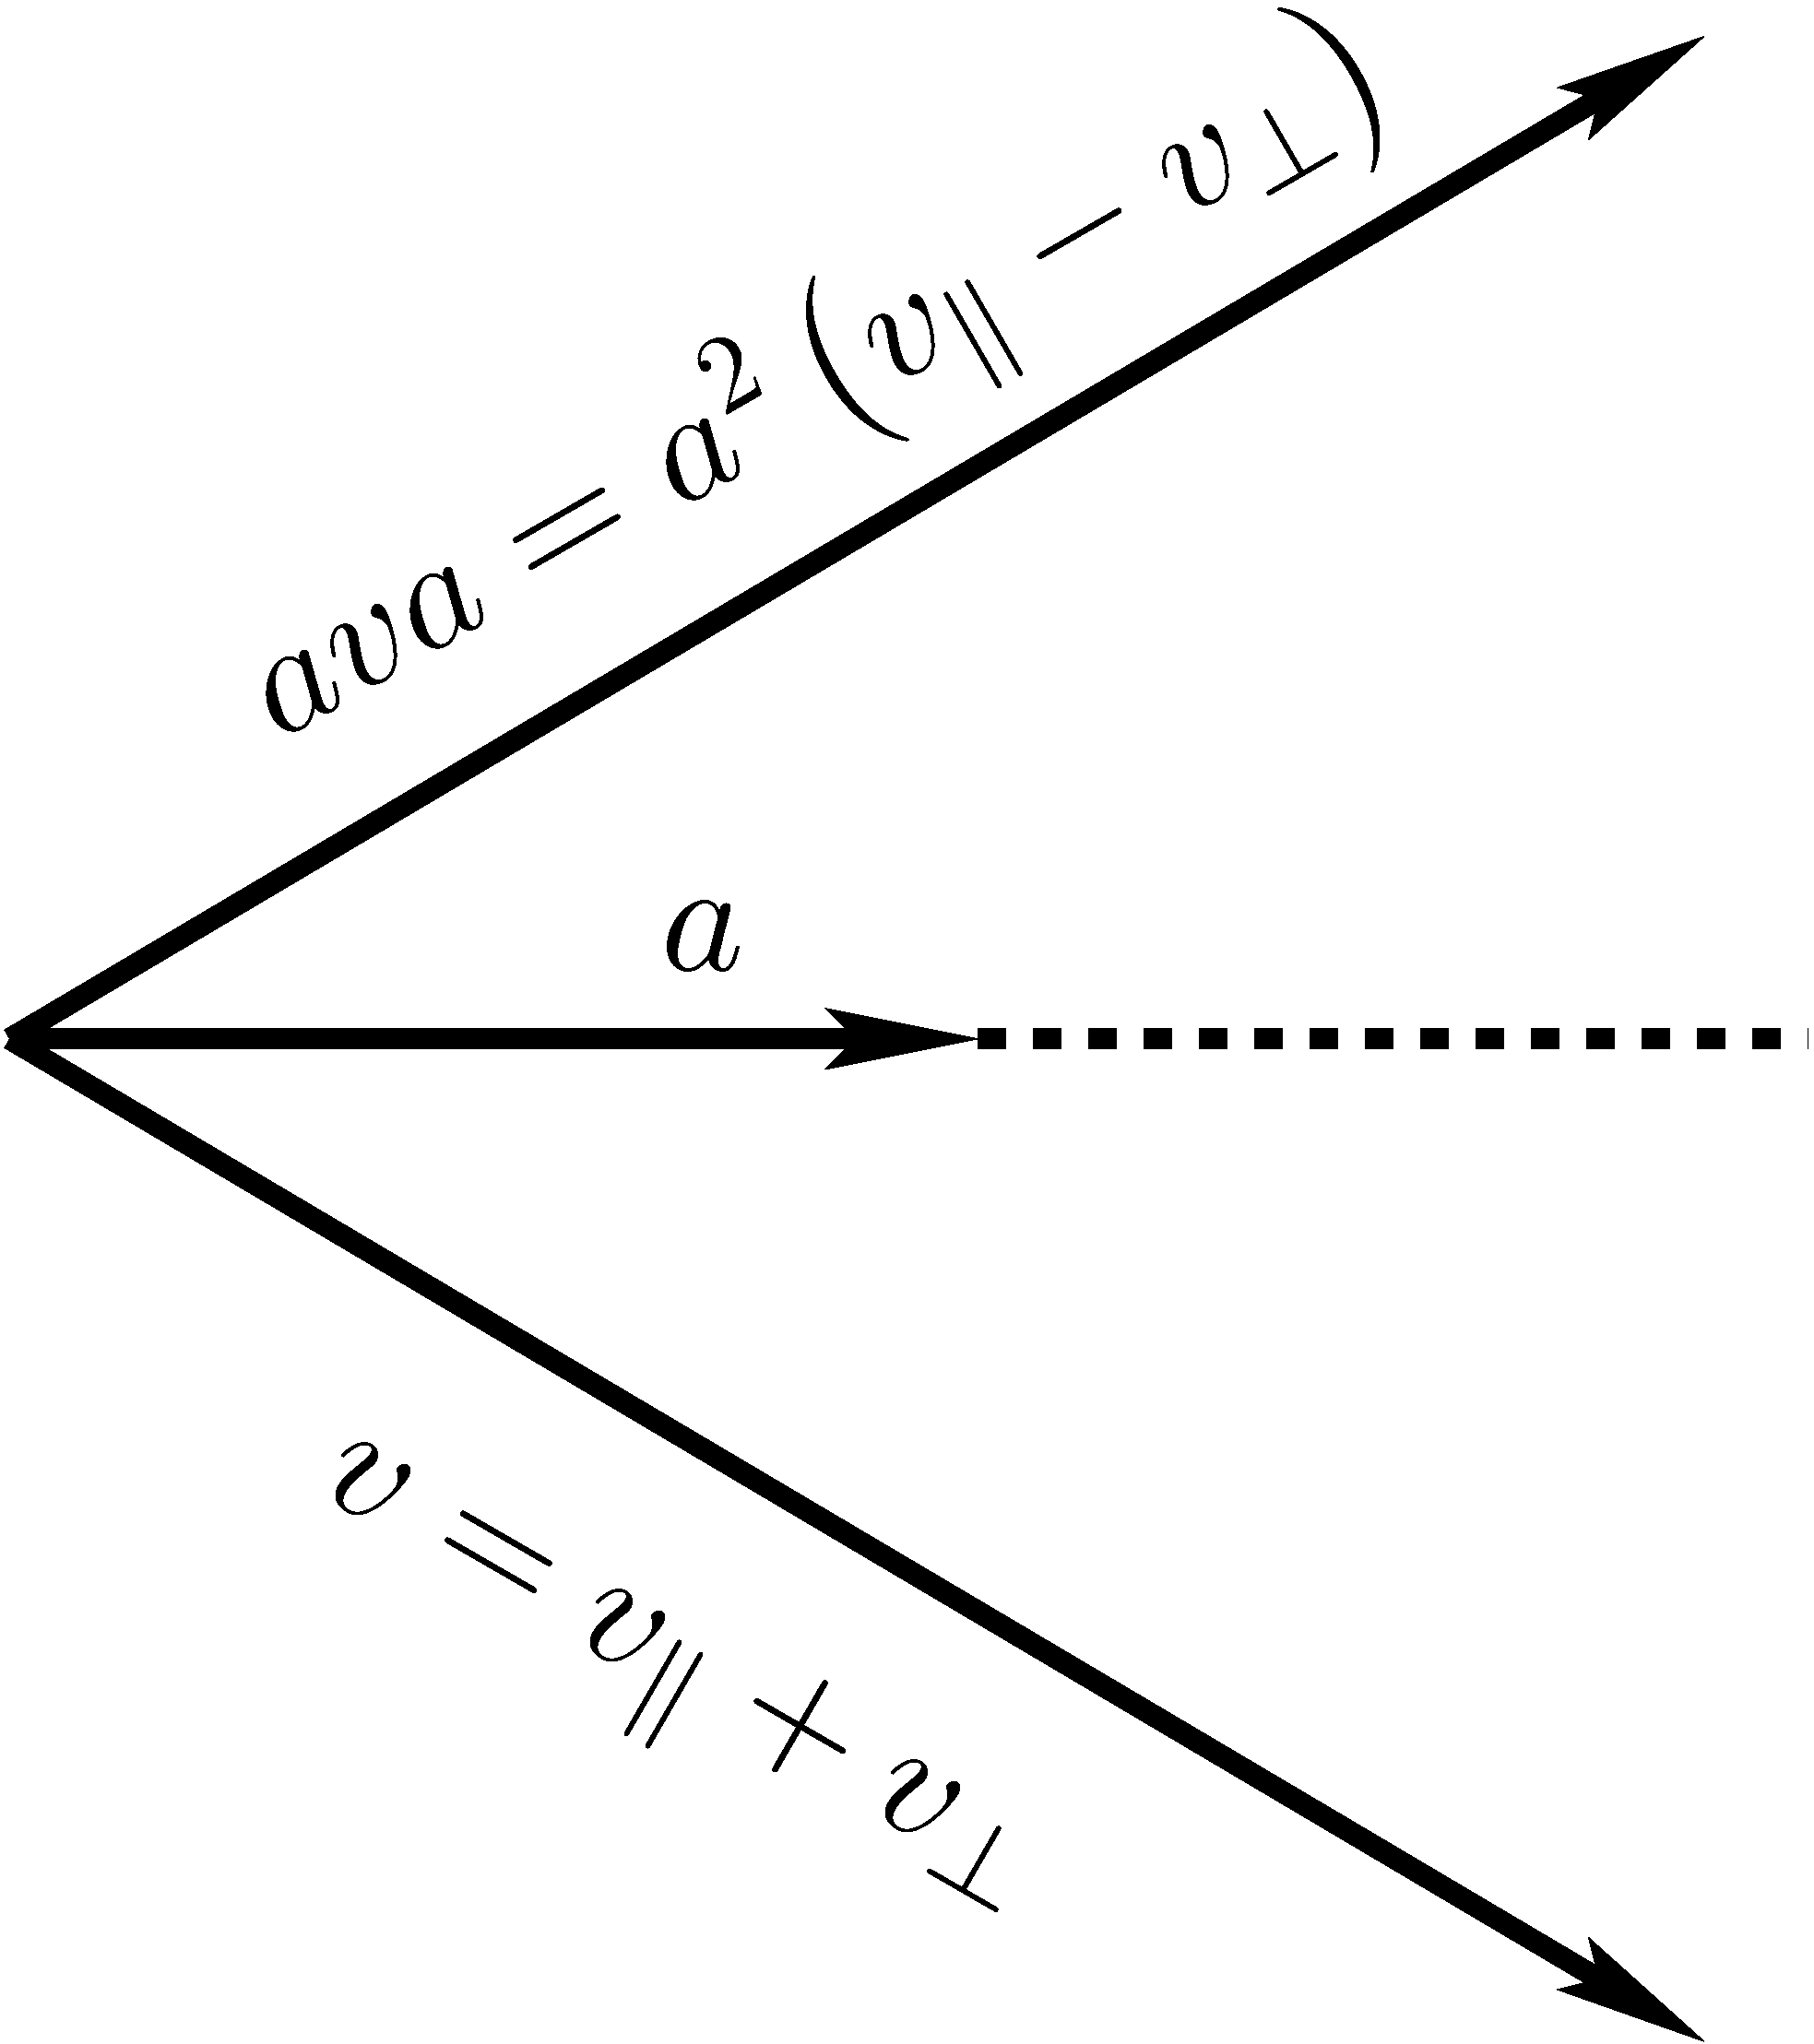
\includegraphics{reflect.png}}
\caption{Reflection of Vector}
\end{center}
\end{figure}
\begin{enumerate}
\item Decompose $v = v_{\parallel}+v_{\perp}$ where $v_{\parallel}$ is the part of $v$
parallel to $a$ and $v_{\perp}$ is the part perpendicular to $a$.
\item $av = av_{\parallel}+av_{\perp} = v_{\parallel}a-v_{\perp}a$ since $a$ and $v_{\perp}$ are
orthogonal.
\item $ava = a^{2}\lp v_{\parallel}-v_{\perp}\rp$ is a vector since $a^{2}$ is a scalar.
\item $ava$ is the reflection of $v$ about the direction of $a$ if $a^{2} = 1$.
\item Thus $\vprod{a_{1}}{a_{r}}v\vprod{a_{r}}{a_{1}} \in \Vsp$ and produces a composition of reflections
of $v$ if $a^{2}_{1} = \dots = a^{2}_{r} = 1$.
\end{enumerate}

\section{Rotations}\label{sec1_10}
\subsection{Definitions}
First define the reverse of a product of vectors. If $R = \vprod{a_{1}}{a_{s}}$ then the reverse is
$R^{\R} = \lp\vprod{a_{1}}{a_{s}}\rp^{\R} = \vprod{a_{r}}{a_{1}}$, the order of multiplication
is reversed. Then let $R = ab$ so that
\be
RR^{\R} = (ab)(ba) = ab^{2}a = a^{2}b^{2} = R^{\R}R
\ee
Let $RR^{\R} = 1$ and calculate $\lp RvR^{\R}\rp^{2}$, where $v$ is an arbitrary vector.
\be
     \lp RvR^{\R}\rp^{2} = RvR^{\R}RvR^{\R} = Rv^{2}R^{\R} = v^{2}RR^{\R} = v^{2}
\ee
Thus $RvR^{\R}$ leaves the length of $v$ unchanged. Now we must also prove $Rv_{1}R^{\R}\cdot R v_{2}R^{\R} = v_{1}\cdot v_{2}$. Since
$Rv_{1}R^{\R}$ and $Rv_{2}R^{\R}$ are both vectors we can use the definition of the
dot product for two vectors
\begin{align*}
Rv_{1}R^{\R}\cdot R v_{2}R^{\R} & = \half\lp Rv_{1}R^{\R}Rv_{2}R^{\R}+Rv_{2}R^{\R}Rv_{1}R^{\R} \rp \\
                              & = \half\lp Rv_{1}v_{2}R^{\R}+Rv_{2}v_{1}R^{\R} \rp  \\
                              & = \half R\lp v_{1}v_{2}+v_{2}v_{1}\rp R^{\R} \\
                              & = R\lp v_{1}\cdot v_{2}\rp R^{\R} \\
                              & = v_{1}\cdot v_{2}RR^{\R} \\
                              & = v_{1}\cdot v_{2}
\end{align*}
Thus the transformation $RvR^{\R}$ preserves both length and angle and must be a rotation. The normal 
designation for $R$ is a rotor.  If we have a series of successive rotations $R_{1},R_{2},\dots,R_{k}$ to be applied to a vector $v$ then
the result of the $k$ rotations will be
$$
	R_{k}R_{k-1}\dots R_{1}vR_{1}^{\R}R_{2}^{\R}\dots R_{k}^{\R}
$$
Since each individual rotation can be written as the geometric product of two vectors, the composition of 
$k$ rotations can be written as the geometric product of $2k$ vectors.  The multivector that results from
the geometric product of $r$ vectors is called a {\bf versor} of order $r$. A composition of rotations is
always a versor of even order.
\subsection{General Rotation}\label{sec1_10_2}
The general rotation can be represented by $R = e^{\thh u}$ where $u$ is a unit
bivector in the plane of the rotation and $\theta$ is the rotation angle in 
the plane.\footnote{$e^{A}$ is defined as the 
Taylor series expansion $e^{A} = {\ds\sum_{j=0}^{\infty}\frac{A^{j}}{j!}}$ where $A$ is any multivector.}
 The two possible non-degenerate cases are $u^{2} = \pm 1$
\be
e^{\thh u} = \left \{
\begin{array}{crl}
\mbox{(Euclidean plane)} & u^{2} = -1: & \cosf{\thh}+u\sinf{\thh} \\
\mbox{(Minkowski plane)} & u^{2} = 1:  & \coshf{\thh}+u\sinhf{\thh} \\
\end{array}
\right \}
\ee
Decompose $v = \vp+\lp v-\vp \rp$ where $\vp$ is the projection of $v$ into the plane defined 
by $u$. Note that $v-\vp$ is orthogonal to all vectors in the $u$ plane. Now let $u = \epep$ where $\epar$ is
parallel to $\vp$ and of course $\eperp$ is in the plane $u$ and orthogonal to $\epar$. $v-\vp$ anticommutes with
$\epar$ and $\eperp$ and $\vp$ anticommutes with $\eperp$ (it is left to the reader to show $RR^{\R} = 1$).

\subsection{Euclidean Case}
For the case of $u^{2} = -1$
\begin{figure}[htbp]
\begin{center}
\scalebox{0.65}{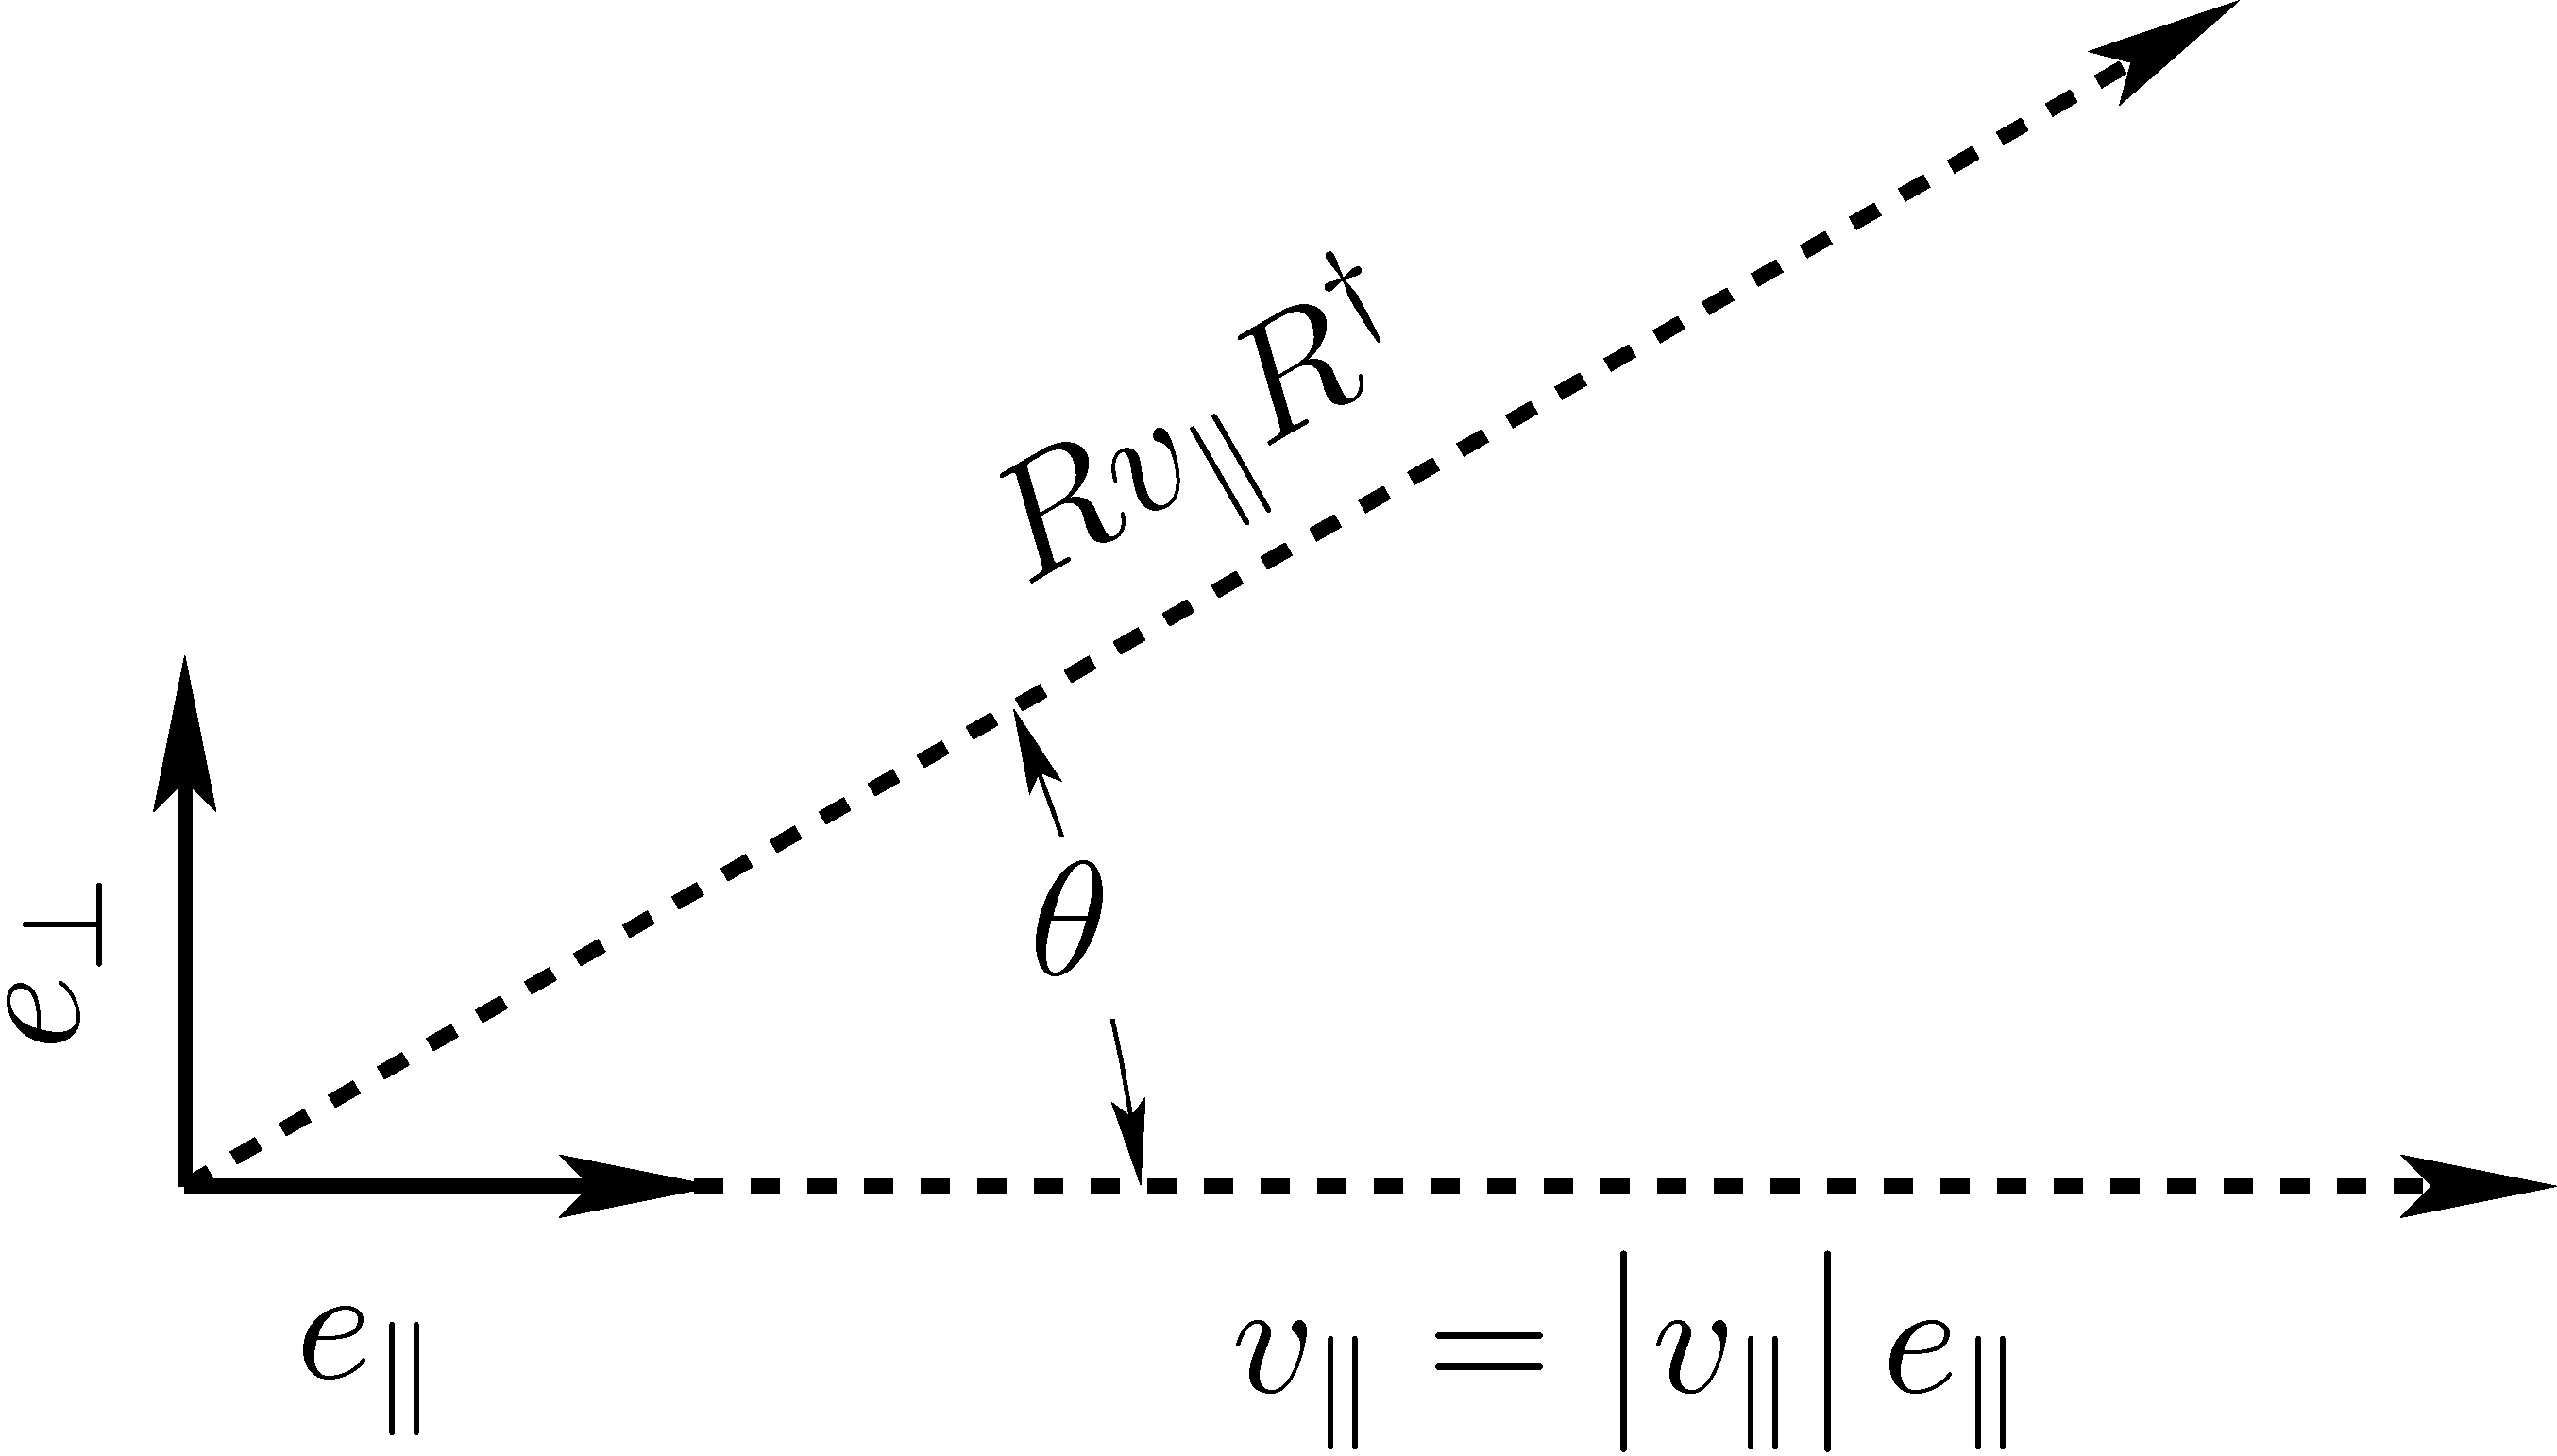
\includegraphics{rotate.png}}
\caption{Rotation of Vector}
\end{center}
\end{figure}

$$
\hspace{-0.5in}RvR^{\R} = \lp \cosf{\thh}+\epep\sinf{\thh}\rp\lp \vp+\lp v-\vp \rp \rp \lp\cosf{\thh}+\epepr\sinf{\thh}\rp
$$

Since $v-\vp$ anticommutes with $\epar$ and $\eperp$ it commutes with $R$ and 
\be
RvR^{\R} = R\vp R^{\R} +\lp v-\vp \rp
\ee
So that we only have to evaluate
\be
\hspace{-0.5in}R\vp R^{\R} =  \lp \cosf{\thh}+\epep\sinf{\thh}\rp\vp\lp\cosf{\thh}+\epepr\sinf{\thh}\rp
\ee
Since $\vp = \abs{\vp}\epar$
\be
R\vp R^{\R} = \abs{\vp}\lp \cosf{\theta}\epar+\sinf{\theta}\eperp \rp
\ee
and the component of $v$ in the $u$ plane is rotated correctly.

\subsection{Minkowski Case}
For the case of $u^{2} = 1$ there are two possibilities, $\vp^{2} > 0$ or $\vp^{2} < 0$.
In the first case $\epar^{2} = 1$ and $\eperp^{2} = -1$. In the second case $\epar^{2} = -1$ 
and $\eperp^{2} = 1$. Again $v-\vp$ is not affected by the rotation so that we need only
evaluate
$$
R\vp R^{\R} =\lp \coshf{\thh}+\epep\sinhf{\thh}\rp\vp\lp\coshf{\thh}+\epepr\sinhf{\thh}\rp
$$
Note that in this case $\abs{\vp} = \sqrt{\abs{\vp^{2}}}$ and
\be
R\vp R^{\R} = \left \{
\begin{array}{c}
\vp^{2} > 0: \abs{\vp}\lp\coshf{\theta}\epar+\sinhf{\theta}\eperp \rp  \\
\vp^{2} < 0: \abs{\vp}\lp\coshf{\theta}\epar-\sinhf{\theta}\eperp \rp  \\
\end{array}
\right \}
\ee
\section{Expansion of geometric product and generalization of $\cdot$ and $\w$}
If $A_{r}$ and $B_{s}$ are respectively grade $r$ and $s$ pure grade multivectors
then
\be\label{21}
\hspace{-0.25in}A_{r}B_{s} = \proj{A_{r}B_{s}}{\abs{r-s}}+\proj{A_{r}B_{s}}{\abs{r-s}+2}+\cdots+
             \proj{A_{r}B_{s}}{\min(r+s,2N-(r+s))}
\ee
\be\label{22}
A_{r}\cdot B_{s} \equiv \proj{A_{r}B_{s}}{\abs{r-s}}
\ee
\be\label{23}
A_{r}\w B_{s} \equiv \proj{A_{r}B_{s}}{r+s}
\ee
Thus if $r+s > N$ then $A_{r}\w B_{s} = 0$, also note that these formulas are the most efficient
way of calculating $A_{r}\cdot B_{s}$ and $A_{r}\w B_{s}$.  Using equations~\ref{17} and \ref{21} we 
can prove that for a vector $a$ and a grade $r$ multivector $B_{r}$
\be\label{24}
     a\cdot B_{r} = \half\paren{aB_{r}-\paren{-1}^{r}B_{r}a}
\ee
\be\label{25}
     a\w B_{r} = \half\paren{aB_{r}+\paren{-1}^{r}B_{r}a}
\ee
If equations~\ref{24} and \ref{25} are true for a grade $r$ blade they are also true for a grade $r$
multivector (superposition of grade $r$ blades). By equation~\ref{17} let 
$B_{r} = \vprod{e_{1}}{e_{r}}$ where the $e's$ are orthogonal and expand $a$ 
\be
a = a_{\perp}+\sum^{r}_{j=1}\alpha_{j}e_{j}
\ee
where $a_{\perp}$ is orthogonal to all the $e's$.
Then\footnote{$e_{1}\dots e_{j-1}\breve{e}_{j}e_{j+1}\dots e_{r} 
= e_{1}\dots e_{j-1}e_{j+1}\dots e_{r}$}
\begin{align}\label{27}
aB_{r} & = \sum^{r}_{j=1}(-1)^{j-1}\alpha_{j}e_{j}^{2}e_{1}\cdots \breve{e}_{j}\cdots e_{r}
              +a_{\perp}\vprod{e_{1}}{e_{r}} \nonumber \\
       & = a\cdot B_{r} + a\w B_{r}
\end{align}
Now calculate
\begin{align}\label{30}
B_{r}a & = \sum^{r}_{j=1}(-1)^{r-j}\alpha_{j}e_{j}^{2}e_{1}\cdots \breve{e}_{j}\cdots e_{r}
           -\paren{-1}^{r-1}a_{\perp}\vprod{e_{1}}{e_{r}} \nonumber \\
       & = \paren{-1}^{r-1}\paren{\sum^{r}_{j=1}(-1)^{j-1}\alpha_{j}e_{j}^{2}e_{1}\cdots \breve{e}_{j}\cdots e_{r}
           -a_{\perp}\vprod{e_{1}}{e_{r}}} \nonumber \\
       & = \paren{-1}^{r-1}\paren{a\cdot B_{r}-a\w B_{r}} 
\end{align}
Adding and subtracting equations~\ref{27} and \ref{30} gives equations~\ref{24} and \ref{25}.
\section{Duality and the Pseudoscalar}
If $e_{1},\dots,e_{n}$ is an orthonormal basis for the vector space the the pseudoscalar $I$ is defined by
\be\label{40}
	I = \vprod{e_{1}}{e_{n}}
\ee
Since one can transform one orthonormal basis to another by an orthogonal transformation the $I$'s for all
orthonormal bases are equal to within a $\pm 1$ scale factor with depends on the ordering of the basis vectors.
If $A_{r}$ is a pure $r$ grade multivector $\paren{A_{r} = \proj{A_{r}}{r}}$ then
\be\label{41}
	A_{r}I = \proj{A_{r}I}{n-r}
\ee
or $A_{r}I$ is a pure $n-r$ grade multivector.  Further by the symmetry properties of $I$ we have
\be\label{42}
	IA_{r} = \paren{-1}^{\paren{n-1}r}A_{r}I
\ee
$I$ can also be used to exchange the $\cdot$ and $\w$ products as follows using equations~\ref{24} and
\ref{25}
\begin{align}
	a\cdot\paren{A_{r}I} & =  \half\paren{aA_{r}I-\paren{-1}^{n-r}A_{r}Ia} \\
						 & =  \half\paren{aA_{r}I-\paren{-1}^{n-r}\paren{-1}^{n-1}A_{r}aI} \\
                         & =  \half\paren{aA_{r}+\paren{-1}^{r}A_{r}a}I \\
						 & = \paren{a\w A_{r}}I \label{25a}
\end{align}

More generally if $A_{r}$ and $B_{s}$ are pure grade multivectors with $r+s \le n$ we have using
equation~\ref{22} and \ref{41}
\begin{align}
	A_{r}\cdot\paren{B_{s}I} & = \proj{A_{r}B_{s}I}{\abs{r-\paren{n-s}}} \\
							 & = \proj{A_{r}B_{s}I}{n-\paren{r+s}} \\
							 & = \proj{A_{r}B_{s}}{r+s}I \\
							 & = \paren{A_{r}\w B_{s}}I
\end{align}
Finally we can relate $I$ to $I^{\R}$ by
\be
	I^{\R} = \paren{-1}^{\frac{n\paren{n-1}}{2}}I
\ee
\section{Reciprocal Frames}
Let $\lst{\eb_{1}}{\eb_{n}}$ be a set of linearly independent vectors that span the vector space that are
not necessarily orthogonal. These vectors define the frame (frame vectors are shown in bold face since they are almost always associated with a particular coordinate system) with volume element
\be
	E_{n} \equiv \wprod{\eb_{1}}{\eb_{n}}
\ee
So that $E_{n} \propto I$.  The reciprocal frame is the set of vectors $\lst{\eb^{1}}{\eb^{n}}$ that satisfy the relation
\be
	\eb^{i}\cdot \eb_{j} = \delta^{i}_{j},\quad \forall i,j = 1,\dots,n
\ee
The $\eb^{i}$ are constructed as follows
\be\label{eq61}
	\eb^{j} = \paren{-1}^{j-1}\eb_{1}\w\eb_{2}\w\dots\w\breve{\eb}_{j}\w\dots\w\eb_{n}E_{n}^{-1}
\ee
So that the dot product is (using equation~\ref{25a} since $E_{n}^{-1} \propto I$)
\begin{align}
	\eb_{i}\cdot\eb^{j} &= \paren{-1}^{j-1}\eb_{i}\cdot\paren{\eb_{1}\w\eb_{2}\w\dots\w\breve{\eb}_{j}
							\w\dots\w\eb_{n}E_{n}^{-1}} \\
 						&= \paren{-1}^{j-1}\paren{\eb_{i}\w\eb_{1}\w\eb_{2}\w\dots\w\breve{\eb}_{j}
							\w\dots\w\eb_{n}}E_{n}^{-1} \\
						&= 0,\quad\forall i \ne j
\end{align}
and
\begin{align}
	\eb_{1}\cdot\eb^{1} & = \eb_{1}\cdot\paren{\wprod{\eb_{2}}{\eb_{n}}E_{n}^{-1}} \\
						& = \paren{\eb_{1}\w\wprod{\eb_{2}}{\eb_{n}}}E_{n}^{-1} \\
						& = 1 
\end{align}
\section{Coordinates}
The reciprocal frame can be used to develop a coordinate representation for multivectors in an arbitrary frame
$\eb_{1},\dots,\eb_{n}$ with reciprocal frame $\eb^{1},\dots,\eb^{n}$.
Since both the frame and it's reciprocal span the base vector space we can write any vector $a$ in the vector space
as
\be
	a = a^{i}\eb_{i} = a_{i}\eb^{i}
\ee
where if an index such as $i$ is repeated it is assumes that the terms with the repeated index will be summed from
$1$ to $n$. Using that $\eb_{i}\cdot\eb^{j} = \delta_{i}^{j}$ we have
\begin{align}
	a_{i} &= a\cdot\eb_{i} \\
	a^{i} &= a\cdot\eb^{i}
\end{align}
In tensor notation $a_{i}$ would be the covariant representation and $a^{i}$ the contravariant representation of the 
vector $a$.  Now consider the case of grade 2 and grade 3 blades:
\begin{align}
	\eb^{i}\cdot\paren{a\w b} &= a\cdot\eb^{i}b-b\cdot\eb^{i}a \nonumber \\
	\eb_{i}\paren{a\cdot\eb^{i}b-b\cdot\eb^{i}a} &= ab-ba = 2a\w b \nonumber \\
	\eb^{i}\cdot\paren{a\w b\w c} &= a\cdot\eb^{i}b\w c-b\cdot\eb^{i}a\w c+ c\cdot\eb^{i}a\w b \nonumber \\
	\eb_{i}\paren{a\cdot\eb^{i}b\w c-b\cdot\eb^{i}a\w c+ c\cdot\eb^{i}a\w b} &= ab\w c-ba\w c+ca\w b = 3a\w b\w c \nonumber 
\end{align}
for an $r$-blade $A_{r}$ we have (the proof is left to the reader)
\be\label{eq71}
	\eb_{i}\eb^{i}\cdot A_{r} = rA_{r}
\ee
Since $\eb_{i}\eb^{i} = n$ we have
\be\label{eq72}
	\eb_{i}\eb^{i}\w A_{r} = \eb_{i}\paren{\eb^{i}A_{r}-\eb^{i}\cdot A_{r}} = \paren{n-r}A_{r}
\ee
Flipping $\eb^{i}$ and $A_{r}$ in equations~\ref{eq71} and \ref{eq72} and subtracting equation~\ref{eq71}
from \ref{eq72} gives
\be
	\eb_{i}A_{r}\eb^{i} = \paren{-1}^{r}\paren{n-2r}A_{r}
\ee
In Hestenes and Sobczyk (3.14) it is proved that
\be
	\paren{\eb^{k_{r}}\w\dots\w\eb^{k_{1}}}\cdot\paren{\eb_{j_{1}}\w\dots\w\eb_{j_{r}}} =
	\delta_{k_{1}}^{j_{1}}\delta_{k_{2}}^{j_{2}}\dots\delta_{k_{r}}^{j_{r}}
\ee
so that the general multivector $A$ can be expanded in terms of the blades of the frame and reciprocal frame as
\be\label{eq1_75}
	A = \sum_{i<j<\cdots<k} A_{ij\cdots k}\eb^{i}\w\eb^{j}\w\cdots\w\eb^{k}
\ee
where
\be\label{eq1_76}
	A_{ij\cdots k} = \paren{\eb_{k}\w\cdots\w\eb_{j}\w\eb_{i}}\cdot A
\ee
The components $A_{ij\cdots k}$ are totally antisymmetric on all indices and are usually referred to
as the components of an {\em antisymmetric tensor}.
\section{Linear Transformations}\label{sec1_15}
\subsection{Definitions}
Let $f$ be a linear transformation on a vector space $f:\Vsp \rightarrow \Vsp$ with 
$\fof{f}{\alpha a+\beta b} = \alpha\fof{f}{a}+\beta\fof{f}{b}$ $\forall a,b \in \Vsp$
and $\alpha,\beta \in \Re$. Then define the action of $f$ on a blade of the geometric
algebra by
\be\label{eq1_77}
\fof{f}{\wprod{a_{1}}{a_{r}}} = \wprod{\fof{f}{a_{1}}}{\fof{f}{a_{1}}}
\ee
and the action of $f$ on any two $A,B \in \GA{\Vsp}$ by
\be
\fof{f}{\alpha A + \beta B} = \alpha\fof{f}{A}+\beta\fof{f}{B}
\ee
Since any multivector $A$ can be expanded as a sum of blades $\fof{f}{A}$ is
defined. This has many consequences. Consider the following definition for the determinant
of $f$, $\fof{\det}{f}$.
\be\label{1_79}
\fof{f}{I} = \fof{\det}{f}I
\ee
First show that this definition is equivalent to the standard definition of the 
determinant (again $\mset{e_{1}}{e_{N}}$ is an orthonormal basis for $\Vsp$).
\be
\fof{f}{e_{r}} = \sum_{s = 1}^{N}a_{rs}e_{s}
\ee
Then
\begin{align}
\fof{f}{I} &= \wprod{\paren{\sum_{s_{1} = 1}^{N}a_{1s_{1}}e_{s}}}
              {\paren{\sum_{s_{N} = 1}^{N}a_{Ns_{N}}e_{s}}} \nonumber \\
           &= \sum_{\mset{s_{1}}{s_{N}}} \vprod{a_{1s_{1}}}{a_{Ns_{N}}}\vprod{e_{s_{1}}}{e_{s_{N}}}
\end{align}
But
\be
\vprod{e_{s_{1}}}{e_{s_{N}}} = \varepsilon_{\vprod{1}{N}}^{\vprod{s_{1}}{s_{N}}}\vprod{e_{1}}{e_{N}}
\ee
so that
\be
\fof{f}{I} = \sum_{\mset{s_{1}}{s_{N}}} \varepsilon_{\vprod{1}{N}}^{\vprod{s_{1}}{s_{N}}}
             \vprod{a_{1s_{1}}}{a_{Ns_{N}}}I
\ee
or
\be
\fof{\det}{f} = \sum_{\mset{s_{1}}{s_{N}}} \varepsilon_{\vprod{1}{N}}^{\vprod{s_{1}}{s_{N}}}
             \vprod{a_{1s_{1}}}{a_{Ns_{N}}}
\ee
which is the standard definition. Now compute the determinant of the product of the linear
transformations $f$ and $g$
\begin{align}
\fof{\det}{fg}I &= \fof{fg}{I} \nonumber \\
               &= \fof{f}{\fof{g}{I}} \nonumber \\
               &= \fof{f}{\fof{\det}{g}I} \nonumber \\
               &= \fof{\det}{g}\fof{f}{I} \nonumber \\
               &= \fof{\det}{g}\fof{\det}{f}I 
\end{align}
or
\be
\fof{\det}{fg} = \fof{\det}{f}\fof{\det}{g}
\ee
Do you have any idea of how miserable that is to prove from the standard definition of determinant?
\subsection{Adjoint}
If $F$ is linear transformation and $a$ and $b$ are two arbitrary vectors the adjoint function, $\adj{F}$, is
defined by
\be
	a\cdot \adjf{F}{b} = b\cdot F\paren{a}
\ee
From the definition the adjoint is also a linear transformation. For an arbitrary frame $\eb_{1},\dots,\eb_{n}$
we have
\be
	\eb_{i}\cdot \adjf{F}{a} = a\cdot F\paren{\eb_{i}}
\ee
So that we can explicitly construct the adjoint as
\begin{align}
	\adjf{F}{a} & = \eb^{i}\paren{\eb_{i}\cdot \adjf{F}{a}} \nonumber \\
	            & = \eb^{i}\paren{a\cdot \f{F}{\eb_{i}}} \nonumber \\
		        & = \eb^{i}\paren{\f{F}{\eb_{i}}\cdot\eb^{j}}a_{j}
\end{align}
so that $\adj{F}_{ij} = F\paren{\eb_{i}}\cdot\eb^{j}$ is the matrix representation of $\adj{F}$ for the 
$\eb_{1},\dots,\eb_{n}$ frame. However
\be
	F\paren{a} = \eb^{i}\paren{F\paren{\eb^{j}}\cdot\eb_{i}}a_{j}
\ee
so that the matrix representation of $F$ is $F_{ij} = F\paren{\eb^{j}}\cdot\eb_{i}$. If the $\eb_{1},\dots,\eb_{n}$ are
orthonormal then $\eb_{j} = \eb^{j}$ for all $j$ and $\adj{F}_{ij} = F_{ji}$ exactly the same as the adjoint in matrices.

Other basic properties of the adjoint are:
\be
	\adj{\adj{F}}\paren{a} = \eb^{i}a\cdot\adjf{F}{\eb_{i}} = \eb^{i}\eb_{i}\cdot F\paren{a} = F\paren{a}
\ee
and
\begin{align}
	\adjf{FG}{a} & = \eb^{i}\lp \eb_{i}\cdot\adjf{FG}{a} \rp \nonumber \\
			     & = \eb^{i}\lp a\cdot\f{F}{\f{G}{\eb_{i}}} \rp \nonumber \\
			     &=  \eb^{i}\lp \adjf{F}{a}\cdot\f{G}{\eb_{i}} \rp \nonumber \\
			     &=  \eb^{i}\lp \eb_{i}\cdot\adjf{G}{\adjf{F}{a}} \rp \nonumber \\
			     &=  \adjf{G}{\adjf{F}{a}} 
\end{align}
so that $\adj{\adj{F}} = F$ and $\adj{FG} = \adj{G}\,\adj{F}$.
A symmetric function is one where $F = \adj{F}$.  As an
example consider $F\adj{F}$
\be
	\adj{F\adj{F}} = \adj{\adj{F}}\,\adj{F} = F\adj{F}
\ee
\subsection{Inverse}
Another linear algebraic relation in geometric algebra is
\be
f^{-1}\paren{A} = \bfrac{I\adjf{f}{I^{-1}A}}{\det\paren{f}}\ \  \forall A \in \GA{\Vsp}\label{eq1_94}
\ee
where $\adj{f}$ is the adjoint transformation defined by $a\cdot\adjf{f}{b} = b\cdot\fof{f}{a}$
 $\forall a,b \in \Vsp$ and you have an explicit formula for the inverse of a linear transformation!
\section{Commutator Product}\label{sec1_16}
The commutator product of two multivectors $A$ and $B$ is defined as
\be
	A\cross B \equiv \half\paren{AB-BA}
\ee
An important theorem for the commutator product is that for a grade 2 multivector, $A_{2} = \proj{A}{2}$,
and a grade $r$ multivector $B_{r} = \proj{B}{r}$ we have
\be\label{eq131}
 A_{2}B_{r} = A_{2}\w B_{r}+A_{2}\cross B_{r}+A_{2}\cdot B_{r}
\ee
From the geometric product grade expansion for multivectors we have
\be
 A_{2}B_{r} = \proj{A_{2}B_{r}}{r+2}+\proj{A_{2}B_{r}}{r}+\proj{A_{2}B_{r}}{\abs{r-2}}	
\ee 
Thus we must show that 
\be
	\proj{A_{2}B_{r}}{r} = A_{2}\cross B_{r}
\ee
Let $e_{1},\dots,e_{n}$ be an orthogonal set for the vector space where $B_{r} = e_{1}\dots e_{r}$ and 
$A_{2} = {\ds \sum_{l<m=2}^{n}\alpha_{lm}e_{l}e_{m}}$ so we can write
\be
A_{2}\cross B_{r} = \paren{\sum_{l<m=2}^{n}\alpha_{lm}e_{l}e_{m}}\cross\paren{e_{1}\dots e_{r}}
\ee 
Now consider the following three cases
\begin{enumerate}
\item $l \mbox{ and } m > r$ where $e_{l}e_{m}e_{1}\dots e_{r} = e_{1}\dots e_{r}e_{l}e_{m}$
\item $l \le r \mbox{ and } m > r$ where $e_{l}e_{m}e_{1}\dots e_{r} = -e_{1}\dots e_{r}e_{l}e_{m}$
\item $l \mbox{ and } m \le r$ where $e_{l}e_{m}e_{1}\dots e_{r} = e_{1}\dots e_{r}e_{l}e_{m}$
\end{enumerate}
For case~1 and 3 $e_{l}e_{m}$ commute with $B_{r}$ and the contribution to the commutator product is zero.  In
case~3 $e_{l}e_{m}$ anticommutes with $B_{r}$ and thus are the only terms that contribute to the commutator.  All
these terms are of grade $r$ and the theorem is proved.  Additionally, the commutator product obeys the Jacobi identity
\be\label{jacobi}
	A\cross\paren{B\cross C} = \paren{A\cross B}\cross C+B\cross\paren{A\cross C}	
\ee
This is important for the geometric algebra treatment of Lie groups and algebras.
